\documentclass{article}

\usepackage{arxiv}
\usepackage[utf8]{inputenc}
\usepackage[T1]{fontenc}
\usepackage{hyperref}
\usepackage{url}
\usepackage{booktabs}
\usepackage{amsmath}
\usepackage{amsfonts}
\usepackage{array}
\usepackage{microtype}
\usepackage{graphicx}
\usepackage{xcolor}

% Bibliography configuration:
% numeric citations, alphabetical order by surname,
% and surname displayed before given names
\usepackage[
    backend=biber,
    style=numeric,
    sorting=nyt,
    sortcites=true,
    giveninits=true,
    maxbibnames=99,
    maxcitenames=2,
    doi=true,
    url=true,
    isbn=false
]{biblatex}

\addbibresource{references_all.bib}

% Display names as: Surname, Given-name initials
\DeclareNameAlias{author}{family-given}
\DeclareNameAlias{editor}{family-given}
\DeclareNameAlias{translator}{family-given}
\DeclareNameAlias{sortname}{family-given}

\graphicspath{{figures/}}

\title{
Can We Trust LLM Self-Explanations?\\
An Empirical Evaluation of Explanation-Support Faithfulness
in Open-Weight Large Language Models
}




\author{
Yash Sakharam Gavade\\
Department of Computer Science\\
Universit\"at Trier\\
Trier, Germany\\
\texttt{s4yagava@uni-trier.de}
}

\begin{document}
\maketitle

\begin{abstract}

Large Language Models (LLMs) increasingly generate natural-language
explanations together with their predictions, but fluent explanations
may not faithfully support the answers they accompany. This paper
presents a controlled evaluation of self-generated explanations from
Qwen~2.5~3B, Llama~3.2~3B, and DeepSeek-R1 Distill Qwen~1.5B on
GSM8K, CommonsenseQA, and StrategyQA.

Each model was evaluated on 100 fixed samples per dataset using a
standardized answer--explanation prompt, producing 900 responses.
Automatic evaluation measured answer accuracy, strict format
compliance, and generation time. A balanced subset of 90 responses was
additionally reviewed for explanation-support faithfulness, logical
consistency, completeness, and failure type.

DeepSeek achieved the strongest GSM8K accuracy at 80\%, while Qwen
performed best on CommonsenseQA at 76\% and StrategyQA at 60\%.
Llama achieved 100\% strict-format success, whereas DeepSeek achieved
85.67\% and required a larger generation budget. Explanations
accompanying correct answers received a mean faithfulness score of
2.64, compared with 0.89 for incorrect answers
($U=1827.0$, $p<0.001$, Cliff's $\delta=0.804$).

All models nevertheless produced unsupported justifications,
hallucinations, logical or arithmetic errors, and
answer--explanation mismatches. The findings indicate that LLM
self-explanations are useful as inspectable behavioral justifications,
but should not be treated as direct evidence of hidden internal
reasoning.

\end{abstract}

\keywords{
Explainable Artificial Intelligence \and
Large Language Models \and
Self-Explanations \and
Explanation Faithfulness \and
Trustworthiness
}



\section{Introduction}

Large Language Models (LLMs) increasingly generate natural-language
explanations alongside their predictions. These explanations can help
users inspect an answer, but their fluency may create an impression of
transparency that is not always justified. In high-stakes settings, a
coherent explanation may increase trust even when it contains
unsupported claims, invalid reasoning, or a conclusion that conflicts
with the final answer
\cite{gunning2019darpa,chang2024survey,schneider2024genxai,
miller2019explanation}.

This motivates an important distinction between
\emph{plausibility} and \emph{faithfulness}. A plausible explanation is
readable and convincing to a human observer. A faithful explanation
should correctly and consistently support the model's stated answer.
A stronger causal notion would require evidence that the explanation
reflects the internal computation responsible for the prediction, which
cannot be established through output inspection alone
\cite{turpin2023language,lanham2023measuring,
parcalabescu2024measuring}. Accordingly, this paper evaluates
\emph{explanation-support faithfulness}: the degree to which a visible
explanation provides correct, consistent, and sufficient support for
the visible final answer.

Previous work has shown that LLMs can produce fluent post-hoc rationales,
biased chains of thought, and explanations that do not reliably track
the basis of their predictions
\cite{madsen2024selfexplanations,paul2024making,
matton2025walk,zaman2025causal}. However, direct comparison across
open-weight models remains difficult because studies often differ in
datasets, prompts, decoding settings, and evaluation criteria.

This study addresses that gap through a controlled comparison of
Qwen~2.5~3B, Llama~3.2~3B, and DeepSeek-R1 Distill Qwen~1.5B.
Each model is evaluated on 100 fixed samples from GSM8K,
CommonsenseQA, and StrategyQA, covering mathematical, commonsense, and
multi-hop yes/no reasoning
\cite{cobbe2021gsm8k,talmor2019commonsenseqa,geva2021strategyqa}.
All models receive the same answer--explanation prompt, and the
evaluation combines automatic scoring, strict format analysis, runtime
measurement, reviewed manual annotation, and statistical comparison.

The study addresses four research questions:

\begin{enumerate}
    \item \textbf{RQ1:} How does answer accuracy vary across models and
    reasoning tasks?

    \item \textbf{RQ2:} How reliably do models follow the required
    answer--explanation format?

    \item \textbf{RQ3:} How does explanation-support faithfulness vary
    by model, dataset, and answer correctness?

    \item \textbf{RQ4:} Which explanation failure patterns occur most
    frequently?
\end{enumerate}

The analysis is guided by three hypotheses:

\begin{itemize}
    \item \textbf{H1:} Model performance will be task-specific rather
    than uniform across datasets.

    \item \textbf{H2:} Correct answers will be accompanied by higher
    explanation-support faithfulness than incorrect answers.

    \item \textbf{H3:} A reasoning-oriented model may achieve stronger
    mathematical performance at the cost of longer runtime and weaker
    format compliance.
\end{itemize}

The main contributions are:

\begin{itemize}
    \item a controlled comparison of three open-weight LLMs across
    three reasoning datasets and 900 responses;

    \item a reproducible evaluation combining answer accuracy, format
    compliance, runtime, and balanced manual explanation analysis;

    \item an empirical analysis of explanation quality, correctness,
    and common failure patterns using statistical and qualitative
    evidence.
\end{itemize}




\section{Related Work}

\subsection{XAI and LLM Self-Explanations}

Explainable Artificial Intelligence (XAI) studies methods for making
model behavior understandable to human users. Classical approaches such
as LIME and SHAP estimate how input features contribute to a prediction
\cite{ribeiro2016trust,lundberg2017unified}. Broader work emphasizes
that explanation quality should be assessed not only through technical
interpretability, but also through user understanding and appropriate
reliance
\cite{lipton2018mythos,molnar2022interpretable,
miller2019explanation,brahman2022human}.

For LLMs, explanations are themselves generated outputs. Chain-of-Thought
prompting and related methods can improve reasoning performance by
eliciting intermediate steps
\cite{wei2022chain,wang2023selfconsistency,zhou2023least,
yao2023tree,chen2023program}. Other approaches use generated rationales
or feedback to improve later attempts
\cite{zelikman2022star,shinn2023reflexion,madaan2023selfrefine}.
However, improved task performance does not imply that the generated
reasoning faithfully represents the computation responsible for the
answer.

\subsection{Evaluating Explanation Faithfulness}

Recent work distinguishes plausible explanations from faithful ones.
Intervention-based studies test whether changing prompts, rationales, or
supporting information changes model behavior in the expected direction
\cite{turpin2023language,lanham2023measuring,zaman2025causal}.
Other studies examine whether self-explanations improve predictions,
remain consistent with final answers, or behave as post-hoc
justifications
\cite{madsen2024selfexplanations,paul2024making,
matton2025walk,parcalabescu2024measuring}.

Complementary research evaluates hallucination, truthfulness, and
uncertainty. SelfCheckGPT compares multiple generations, semantic
uncertainty aggregates meaning-level variation, and TruthfulQA shows
that fluent outputs may still reproduce false claims
\cite{manakul2023selfcheckgpt,farquhar2024semantic,
lin2022truthfulqa}. Mechanistic interpretability provides a stronger
standard by examining internal circuits and learned features, but such
methods remain difficult to scale to complete model behaviors
\cite{elhage2021framework,bricken2023monosemanticity,
cunningham2024sparse,rai2024practical}.

Because automatic metrics may overlook contradictions,
answer--explanation mismatches, and incomplete reasoning, human or
reviewed behavioral evaluation remains valuable
\cite{celikyilmaz2020evaluation,ma2024openhexai,
mills2025almanacs}. The present study therefore treats explanations as
observable behavioral justifications rather than direct evidence of
hidden causal reasoning.

\subsection{Research Gap}

Existing studies often differ in model access, prompt design, datasets,
decoding settings, and faithfulness criteria, making direct comparison
difficult. Many also focus on either answer accuracy or explanation
quality without jointly examining format compliance, runtime, and
failure patterns.

This work addresses that gap through a fixed benchmark, deterministic
decoding, a common output parser, and the same reviewed scoring rubric
across three open-weight models and three reasoning tasks. The objective
is not to claim access to internal reasoning, but to evaluate whether
visible explanations provide reliable support for visible answers.




\section{Methodology}

\subsection{Models and Datasets}

The study evaluates three compact open-weight instruction models:
Qwen~2.5~3B, Llama~3.2~3B, and DeepSeek-R1 Distill Qwen~1.5B
\cite{qwen2024qwen25,grattafiori2024llama3,deepseek2025r1}.
All models were loaded using 4-bit NF4 quantization to fit within the
available 4\,GB GPU memory.

The benchmark contains 100 fixed examples from each of three datasets:

\begin{itemize}
    \item \textbf{GSM8K}, representing mathematical word-problem
    reasoning \cite{cobbe2021gsm8k};

    \item \textbf{CommonsenseQA}, representing five-option commonsense
    reasoning \cite{talmor2019commonsenseqa};

    \item \textbf{StrategyQA}, representing multi-hop binary reasoning
    \cite{geva2021strategyqa}.
\end{itemize}

GSM8K examples were drawn from the test split, CommonsenseQA examples
from the validation split, and StrategyQA examples from the available
training split. Sampling used random seed 42, and the same 300 questions
were presented to every model.

\subsection{Prompting and Inference}

Each model received the same structured instruction and was required to
produce:

\begin{quote}
\texttt{FINAL\_ANSWER: <answer>}\\
\texttt{EXPLANATION: <concise justification>}
\end{quote}

The expected answer format was numerical for GSM8K, an option label for
CommonsenseQA, and yes/no for StrategyQA. The final answer was requested
before the explanation to support consistent parsing across models.

Greedy decoding was used with sampling disabled and random seed 42.
Qwen and Llama used a maximum of 256 new tokens. DeepSeek used 768 new
tokens because shorter runs frequently ended before both required fields
were produced. Complete model identifiers, hardware details, and
generation settings are reported in Appendix~\ref{app:configuration}.

The evaluation produced:

\[
3\ \text{models}
\times
3\ \text{datasets}
\times
100\ \text{samples}
=
900\ \text{responses}.
\]

Figure~\ref{fig:pipeline} summarizes the experimental pipeline.

\begin{figure}[t]
    \centering
    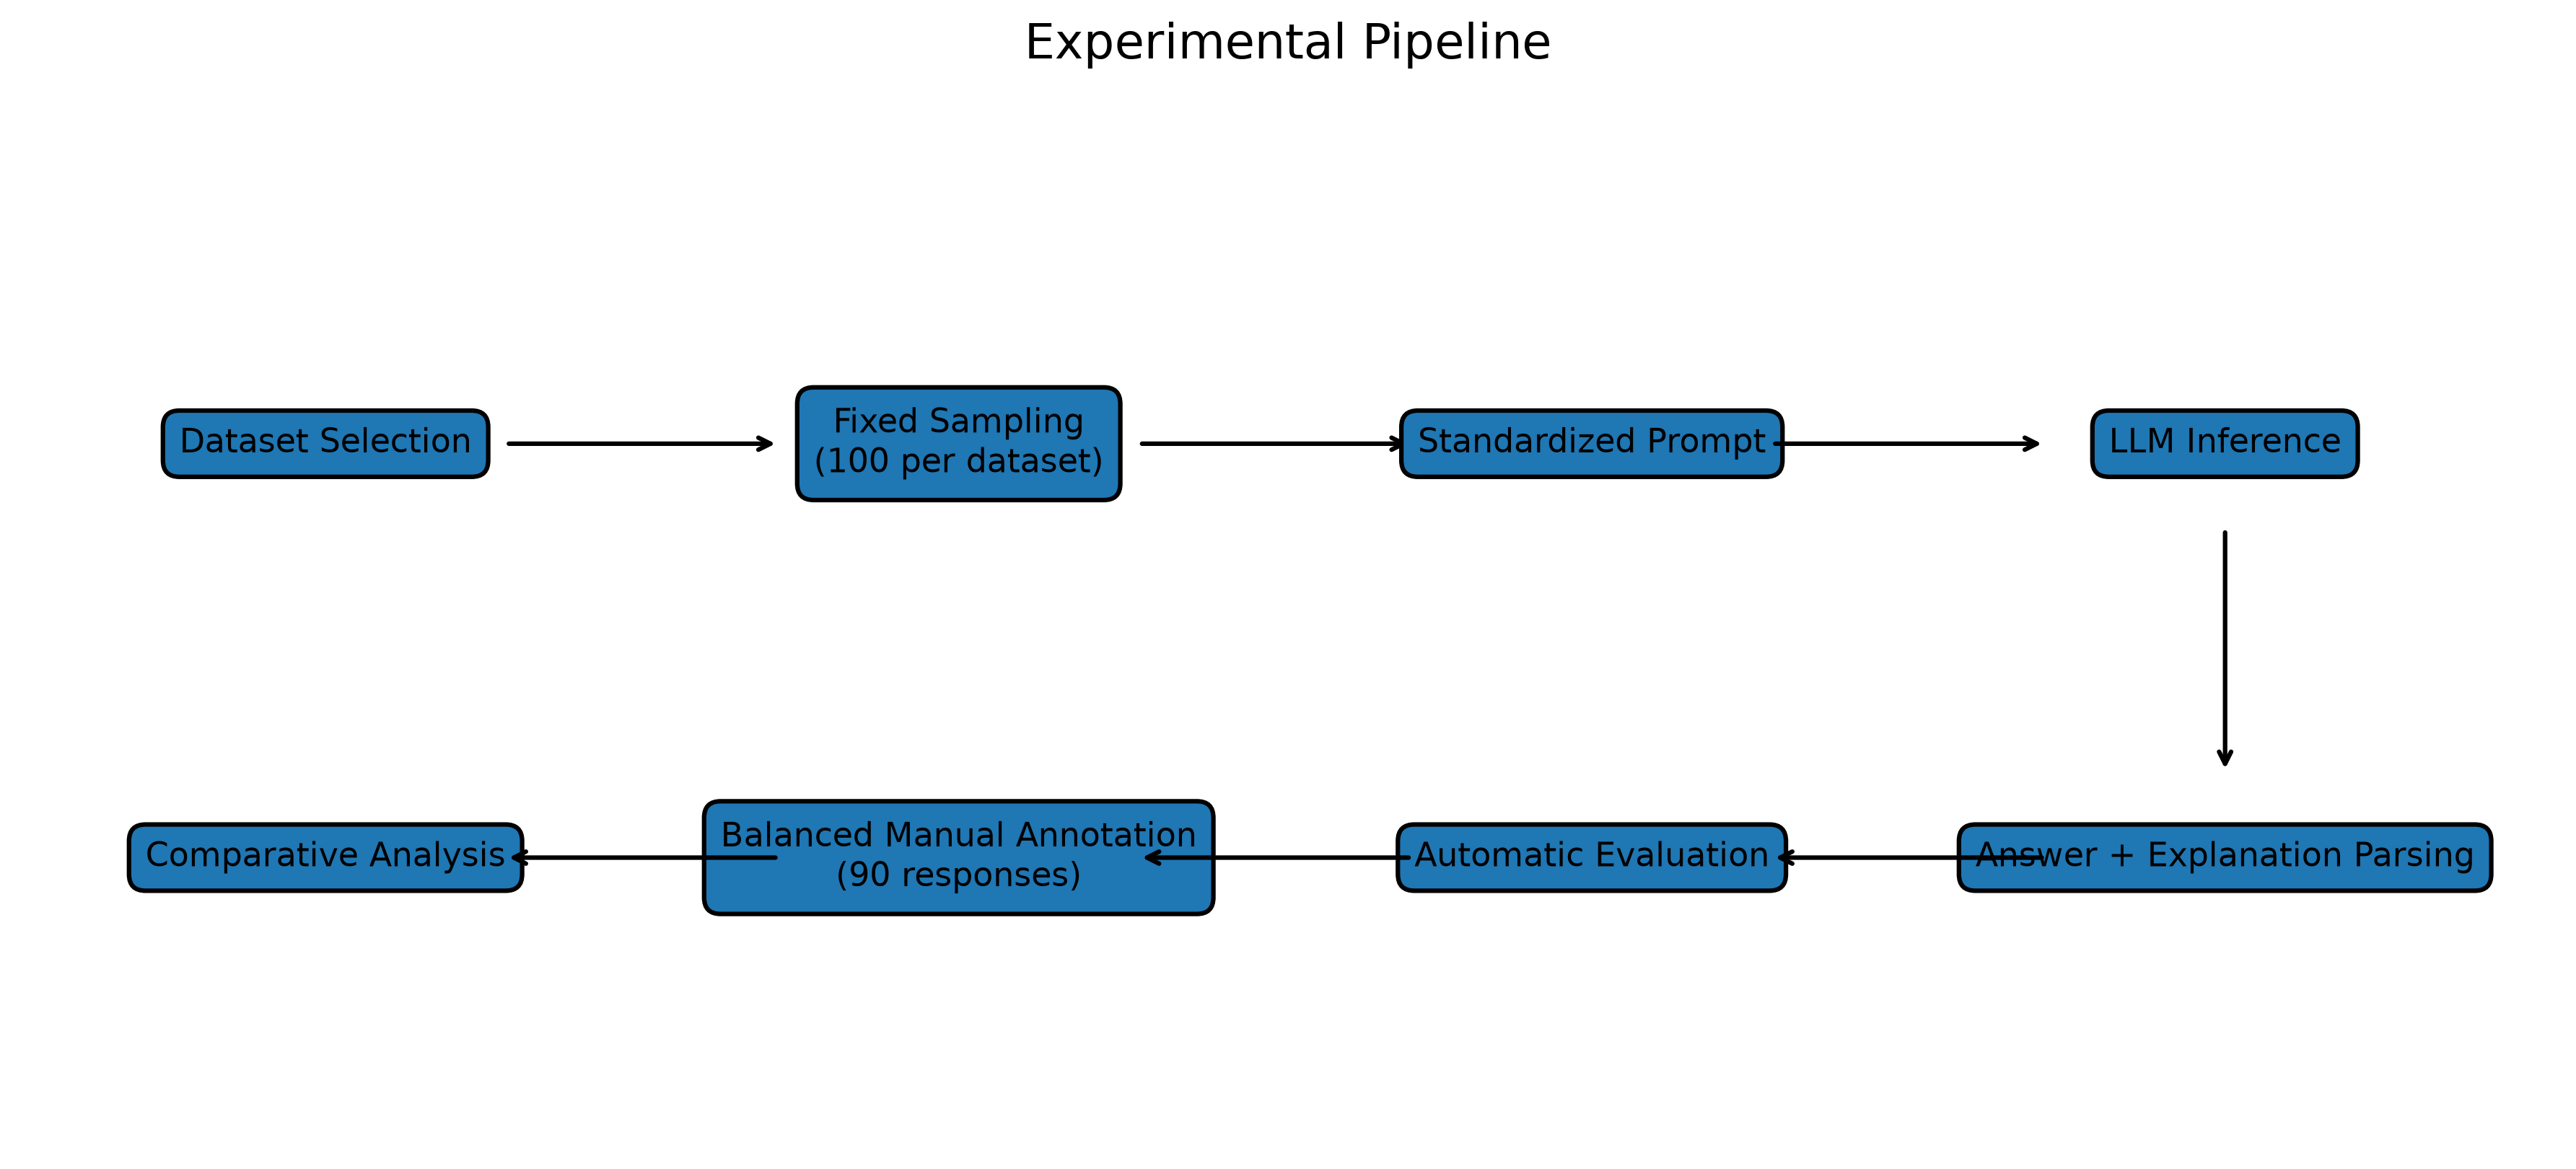
\includegraphics[width=\linewidth]{experimental_pipeline.png}
    \caption{Experimental pipeline for benchmark construction,
    generation, automatic scoring, and reviewed manual analysis.}
    \label{fig:pipeline}
\end{figure}

\subsection{Automatic Evaluation}

A strict parser extracted the required final-answer and explanation
fields. Strict parse success was recorded separately from answer
correctness so that format compliance could be evaluated directly.

Answers were normalized using dataset-specific rules:

\begin{itemize}
    \item numerical normalization for GSM8K;
    \item option-label normalization for CommonsenseQA;
    \item mapping among equivalent yes/no, true/false, and A/B forms for
    StrategyQA.
\end{itemize}

The automatic evaluation measured:

\begin{itemize}
    \item answer accuracy;
    \item strict parse success;
    \item mean generation time;
    \item explanation length.
\end{itemize}

Wilson 95\% confidence intervals were calculated for dataset-level and
overall accuracy.

\subsection{Manual Explanation Analysis}

A balanced subset of 90 successfully parsed responses was selected for
reviewed manual analysis. The sample contained 10 responses for every
model--dataset combination, including five correct and five incorrect
answers whenever possible.

Each explanation was scored from 0 to 3 on:

\begin{itemize}
    \item \textbf{explanation-support faithfulness}: whether the
    explanation correctly supports the stated final answer;

    \item \textbf{logical consistency}: whether the reasoning is coherent
    and free from contradiction;

    \item \textbf{completeness}: whether the explanation contains
    sufficient support for the answer.
\end{itemize}

A primary failure category was additionally assigned, including
answer--explanation mismatch, arithmetic error, contradictory
explanation, factual hallucination, incomplete reasoning,
instruction-following failure, logical error, unsupported justification,
other, or no primary failure. The complete rubric and category
definitions are provided in Appendix~\ref{app:annotation}.

The analysis measures visible behavioral support rather than causal
faithfulness. It does not establish that the explanation reproduces the
hidden internal computation responsible for the answer
\cite{turpin2023language,lanham2023measuring,
parcalabescu2024measuring}.

\subsection{Statistical Analysis}

Because the manual scores are ordinal, correct and incorrect responses
were compared using a two-sided Mann--Whitney U test. Cliff's delta was
reported as a non-parametric effect-size measure. A bootstrap procedure
with 10,000 resamples and random seed 42 estimated a 95\% confidence
interval for the difference in mean faithfulness scores.

The statistical analysis was performed across all 90 reviewed responses
and separately for each model. Complete model-level results are reported
in Appendix~\ref{app:statistics}.

\subsection{Code and Reproducibility}

The source code, experiment configuration, data-preparation scripts,
evaluation scripts, manual-analysis files, and figure-generation code
are available at:

\begin{center}
\url{https://github.com/Yash-Gavade/FaithfulLLM}
\end{center}

Where licensing and storage constraints permit, processed benchmark
metadata and generated outputs are also included. Additional
reproduction details are provided in
Appendix~\ref{app:reproducibility}.





\section{Results}

\subsection{Accuracy and Efficiency}

Table~\ref{tab:main_results} summarizes answer accuracy, strict parse
success, and mean generation time. Figure~\ref{fig:accuracy_ci} shows
dataset-level accuracy with Wilson 95\% confidence intervals.

\begin{table}[t]
\centering
\small
\caption{Answer accuracy, strict parse success, and mean generation
time.}
\label{tab:main_results}
\begin{tabular}{lrrrrrr}
\toprule
\textbf{Model} &
\textbf{GSM} &
\textbf{CSQA} &
\textbf{SQA} &
\textbf{Overall} &
\textbf{Parse} &
\textbf{Time} \\
&
\textbf{(\%)} &
\textbf{(\%)} &
\textbf{(\%)} &
\textbf{(\%)} &
\textbf{(\%)} &
\textbf{(s)} \\
\midrule
Qwen 2.5 3B &
13 & 76 & 60 & 49.67 & 99.33 & 10.21 \\

Llama 3.2 3B &
6 & 70 & 59 & 45.00 & 100.00 & 7.57 \\

DeepSeek-R1 Distill &
80 & 28 & 49 & 52.33 & 85.67 & 37.01 \\
\bottomrule
\end{tabular}
\end{table}

\begin{figure}[t]
    \centering
    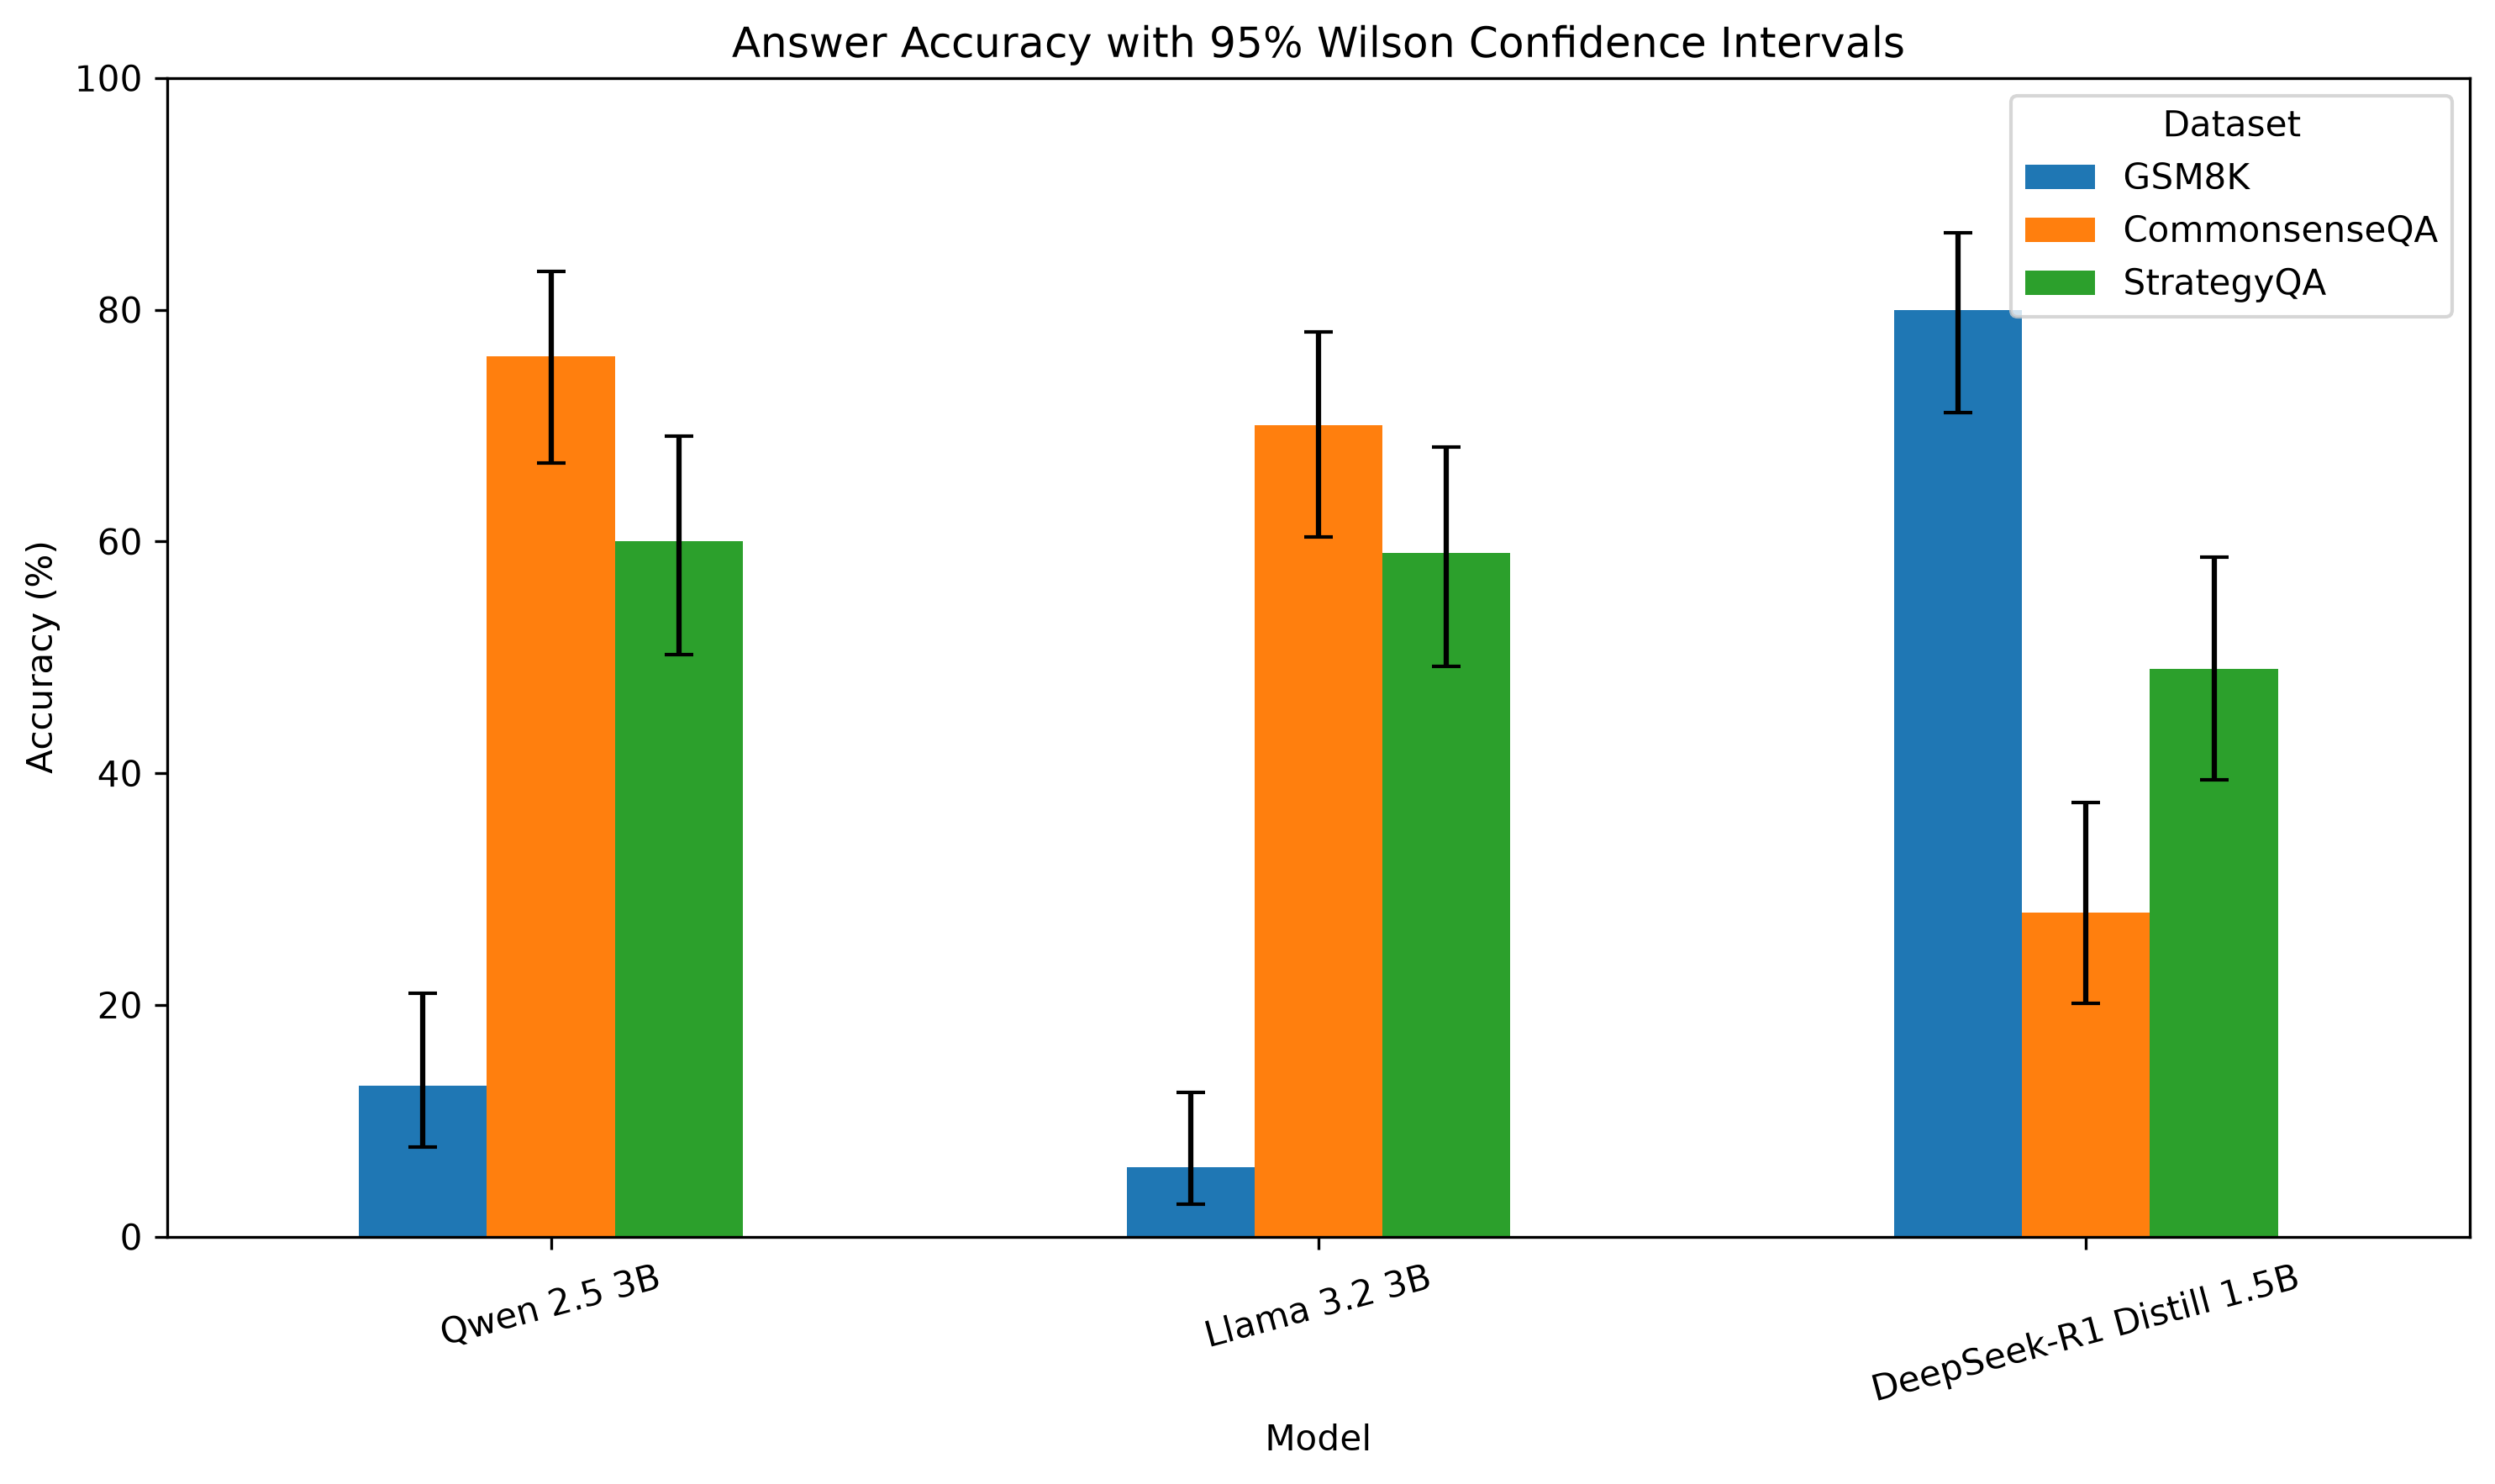
\includegraphics[width=\linewidth]
    {accuracy_with_confidence_intervals.png}
    \caption{Answer accuracy by model and dataset with Wilson 95\%
    confidence intervals. Each dataset-level estimate is based on 100
    samples.}
    \label{fig:accuracy_ci}
\end{figure}

The results show pronounced task specialization. DeepSeek-R1 Distill
achieved 80\% accuracy on GSM8K, substantially outperforming Qwen
(13\%) and Llama (6\%). Qwen achieved the highest observed accuracy on
CommonsenseQA (76\%) and StrategyQA (60\%), followed closely by Llama
on both tasks.

DeepSeek obtained the highest observed overall accuracy at 52.33\%,
followed by Qwen at 49.67\% and Llama at 45.00\%. However, the
corresponding overall confidence intervals overlap, so the aggregate
differences should not be interpreted as decisive evidence of universal
superiority. Complete confidence intervals are reported in
Appendix~\ref{app:accuracy}.

Llama achieved perfect strict-format compliance and the fastest mean
generation time. DeepSeek was substantially slower and less reliable
in producing both required output fields. Its stronger GSM8K
performance therefore came with a practical cost in runtime and format
compliance. Because DeepSeek used a larger generation budget, runtime
should be interpreted as a system-level rather than equal-token
comparison.

\subsection{Explanation Quality}

Table~\ref{tab:manual_scores} reports mean explanation scores across 30
reviewed responses per model.

\begin{table}[t]
\centering
\small
\caption{Mean reviewed explanation scores on a 0--3 scale.}
\label{tab:manual_scores}
\begin{tabular}{lrrr}
\toprule
\textbf{Model} &
\textbf{Faithfulness} &
\textbf{Logic} &
\textbf{Completeness} \\
\midrule
DeepSeek-R1 Distill & 1.87 & 2.07 & 2.03 \\
Llama 3.2 3B & 1.70 & 2.20 & 2.17 \\
Qwen 2.5 3B & 1.73 & 2.13 & 2.30 \\
\bottomrule
\end{tabular}
\end{table}

DeepSeek obtained the highest mean explanation-support faithfulness
score, Llama the highest logical-consistency score, and Qwen the highest
completeness score. These differences are moderate and do not support
the conclusion that one model is uniformly best across all explanation
dimensions.

Explanation quality also varied by dataset. DeepSeek performed strongly
on GSM8K and CommonsenseQA but obtained its lowest faithfulness score on
StrategyQA. The complete model--dataset faithfulness heatmap is reported
in Appendix~\ref{app:additional_figures}.

\subsection{Correctness and Faithfulness}

Figure~\ref{fig:correct_incorrect} compares explanation-support
faithfulness for correct and incorrect answers.

\begin{figure}[t]
    \centering
    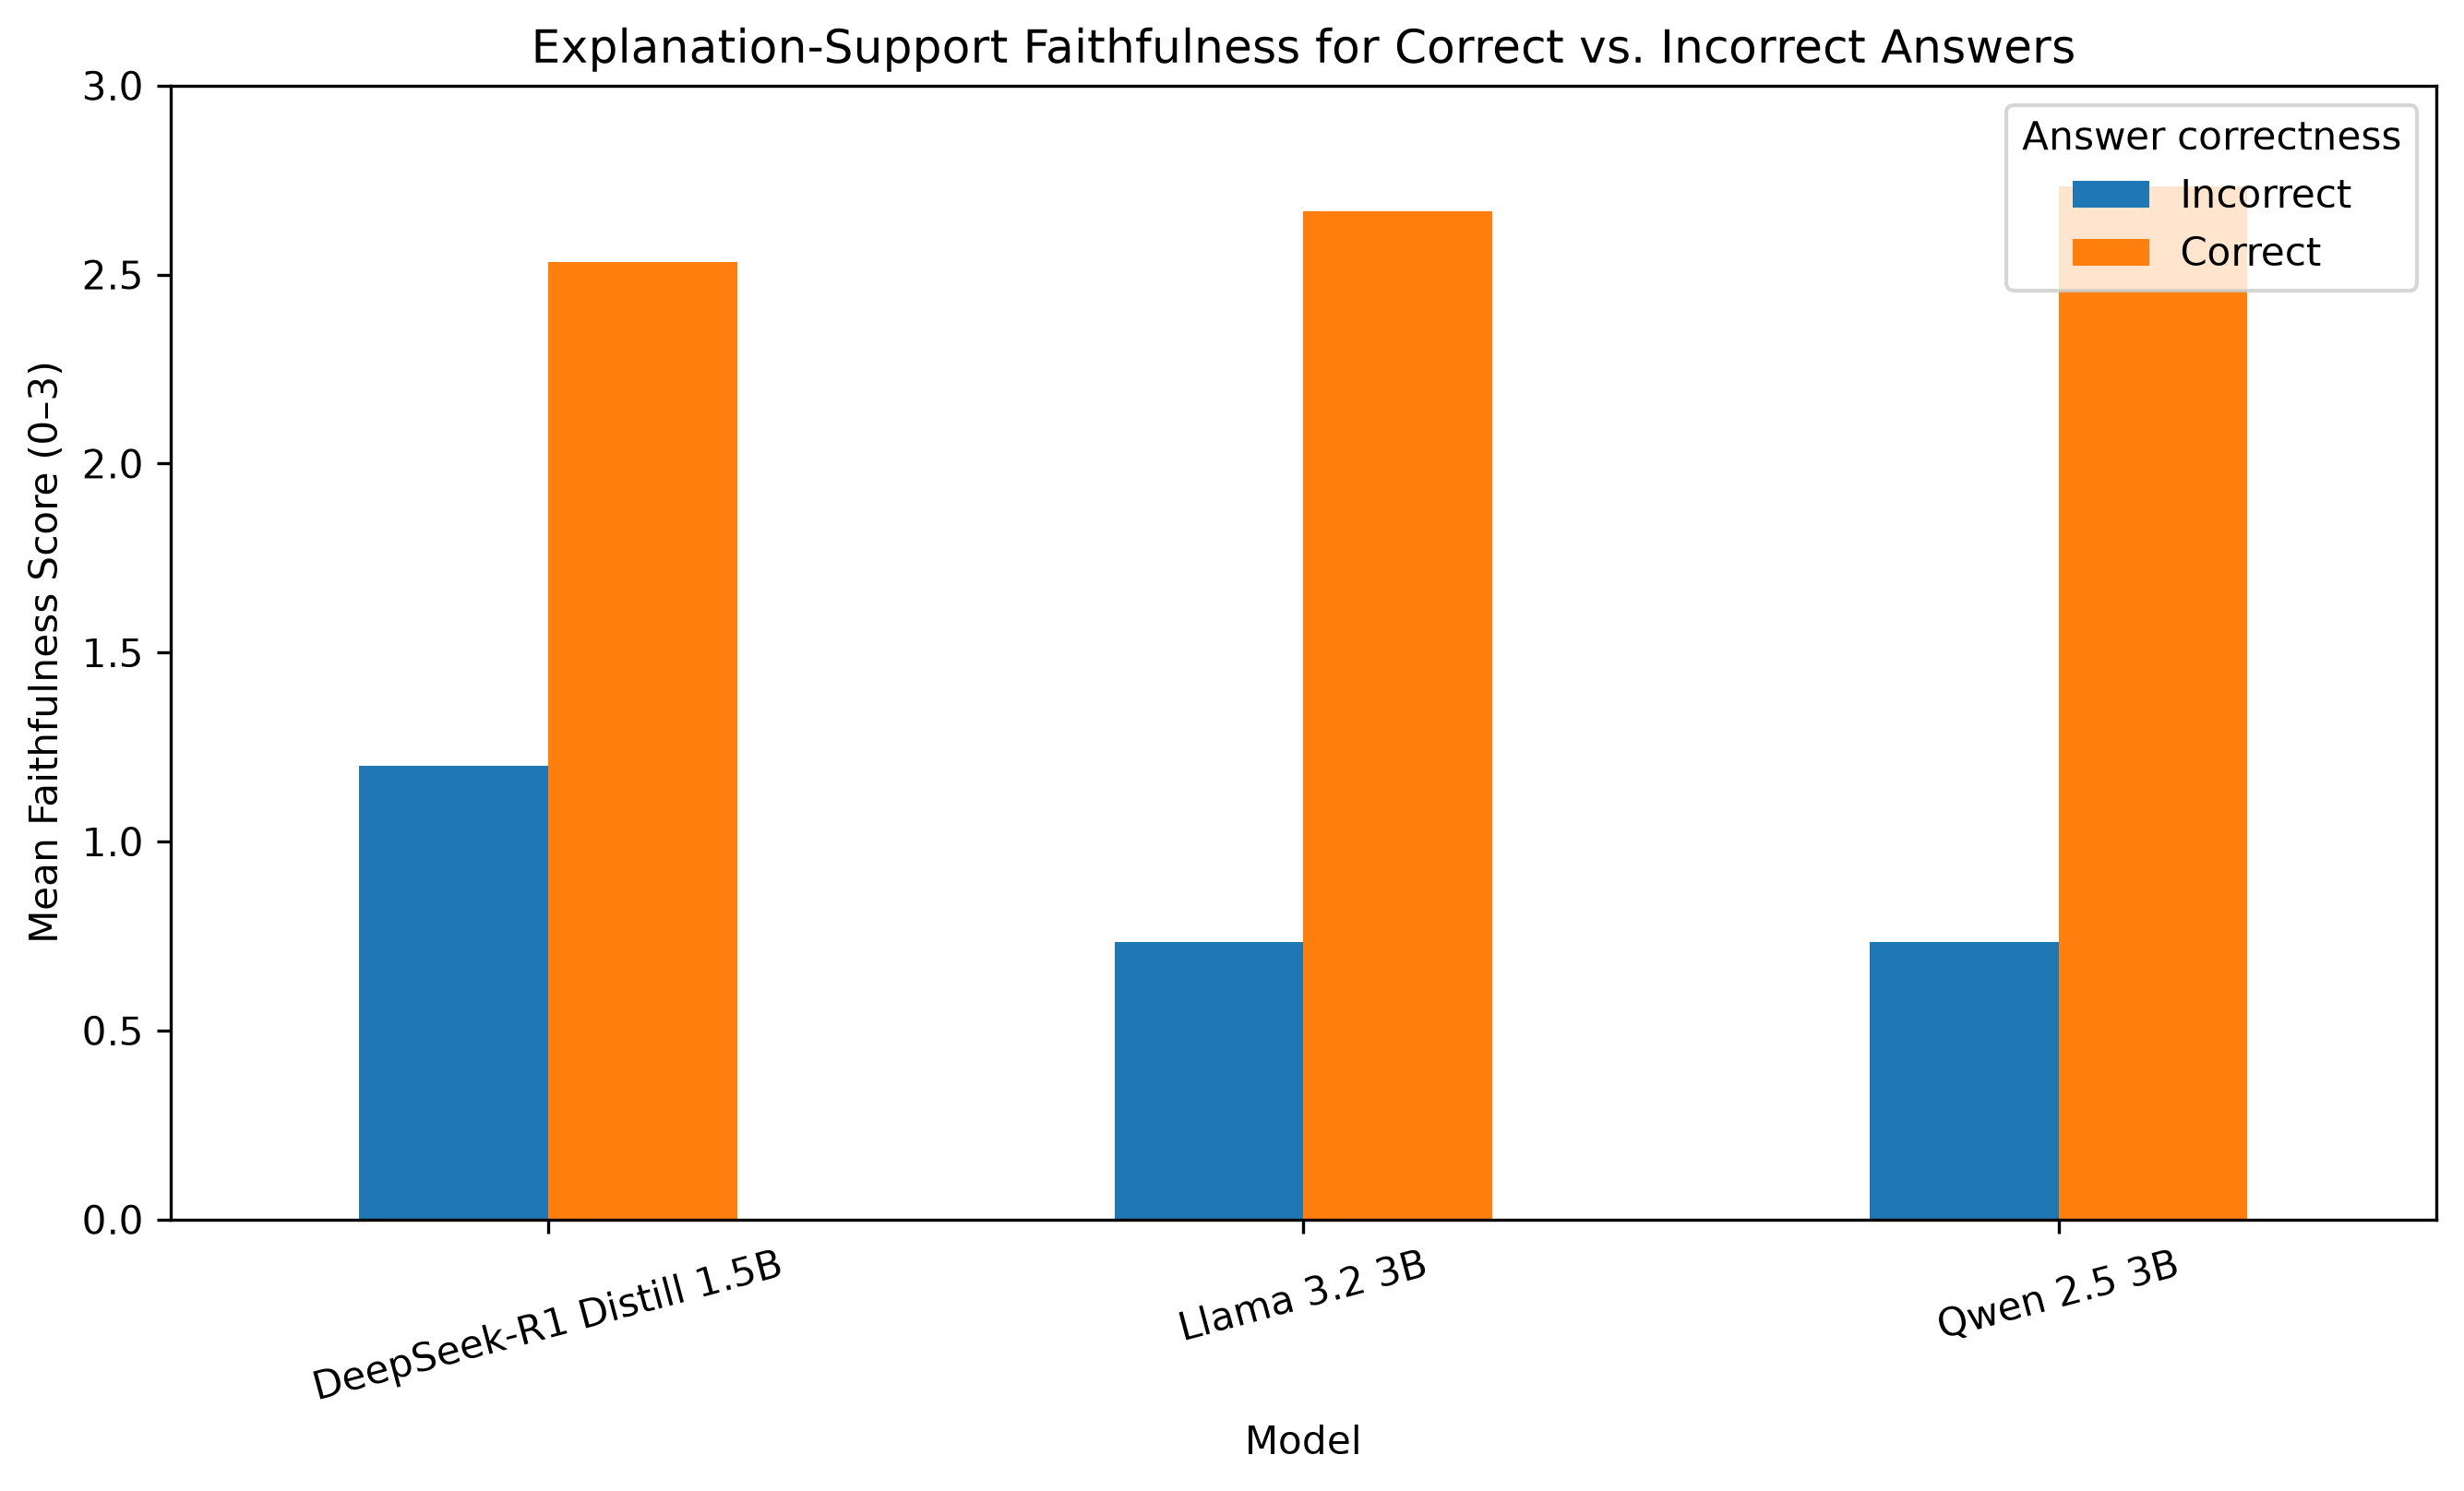
\includegraphics[width=\linewidth]
    {faithfulness_correct_vs_incorrect.png}
    \caption{Mean explanation-support faithfulness for correct and
    incorrect answers.}
    \label{fig:correct_incorrect}
\end{figure}

Across all models, explanations accompanying correct answers received a
mean faithfulness score of 2.64, compared with 0.89 for explanations
accompanying incorrect answers. The mean difference was 1.76 points,
with a bootstrap 95\% confidence interval of [1.42, 2.07].

A two-sided Mann--Whitney U test showed a significant difference between
the distributions
($U=1827.0$, $p<0.001$), and Cliff's delta was 0.804, indicating a
large effect. The same direction of effect was observed for all three
models. Complete model-level statistics are provided in
Appendix~\ref{app:statistics}.

These findings support H2: correct answers are strongly associated with
better visible explanation support. Nevertheless, correctness does not
establish that the explanation reflects the hidden internal computation
responsible for the answer.

\subsection{Failure Analysis}

The reviewed responses contained unsupported justifications, factual
hallucinations, logical and arithmetic errors, contradictory reasoning,
and answer--explanation mismatches. A particularly important failure
occurred when an explanation derived one numerical result but the
reported final answer contained a different value. In another case, a
model selected an incorrect CommonsenseQA option while producing a
fluent but unsupported justification.

These examples show that explanation fluency and answer correctness
must be evaluated separately. The full failure-category distribution is
reported in Appendix~\ref{app:additional_figures}, and representative
qualitative examples are provided in
Appendix~\ref{app:qualitative}.


\section{Discussion}

\subsection{Task-Specific Performance}

The results show that no model is consistently best across all tasks.
DeepSeek-R1 Distill is strongly specialized for mathematical reasoning,
whereas Qwen and Llama perform better on commonsense and strategy
questions. This supports H1 and reinforces broader findings that model
rankings vary substantially across reasoning and knowledge benchmarks
\cite{liang2023helm,hendrycks2021mmlu,
srivastava2023bigbench,zellers2019hellaswag}.

The same trade-off appears in efficiency and instruction following.
DeepSeek's stronger GSM8K performance was accompanied by a larger token
budget, longer generation time, and lower strict-format success. Llama,
by contrast, produced the fastest and most consistently formatted
outputs but achieved the weakest mathematical accuracy. Model selection
should therefore be task-specific and should consider accuracy,
reliability, and computational cost together.

\subsection{Faithfulness and Answer Correctness}

Correct answers were accompanied by substantially higher
explanation-support faithfulness scores than incorrect answers, supporting
H2. However, answer correctness and explanation quality remain distinct.
Some correct answers were supported by incomplete reasoning, while some
incorrect answers were presented with fluent and confident
justifications.

This result is consistent with prior studies showing that generated
rationales may be plausible without faithfully tracking the basis of a
prediction
\cite{turpin2023language,lanham2023measuring,
madsen2024selfexplanations,paul2024making,matton2025walk}.
The observed answer--explanation mismatches are especially important
because a user may accept a convincing explanation without noticing that
it conflicts with the reported answer.

The failure taxonomy further shows that explanation errors are not
uniform. Unsupported justification, factual hallucination, contradictory
reasoning, and arithmetic or logical error represent different trust
risks. This supports the use of multiple evaluation dimensions rather
than a single explanation-quality score
\cite{manakul2023selfcheckgpt,farquhar2024semantic,
siegel2024probabilities,terentowicz2025unfaithful}.

\subsection{Implications for Trustworthy XAI}

The manual scores used in this study evaluate whether a visible
explanation supports a visible answer. They do not establish that the
explanation reveals the internal computation that produced the
prediction. The explanations should therefore be interpreted as
behavioral justifications rather than causal traces of hidden reasoning.

Mechanistic interpretability provides a stronger basis for claims about
internal computation by examining model circuits, features, and
representations
\cite{elhage2021framework,bricken2023monosemanticity,
cunningham2024sparse,rai2024practical}. Such methods were outside the
scope of this study, but they clarify the limits of output-only
faithfulness analysis.

Behavioral explanations can still be useful when treated cautiously.
They allow users and developers to inspect outputs, identify
contradictions, and detect unsupported reasoning. For trustworthy use,
self-explanations should be combined with answer verification,
uncertainty or hallucination estimation, calibration, retrieval
grounding, and explicit consistency checking
\cite{weng2023selfverification,manakul2023selfcheckgpt,
farquhar2024semantic,desai2020calibration,sui2025fidelis}.

Accordingly, four practical conclusions follow: models should be chosen
for the target task rather than by aggregate accuracy alone; generated
explanations should be checked against the final answer; reasoning
models should be evaluated for runtime and truncation as well as
accuracy; and in high-stakes settings, self-explanations should be
treated as supporting evidence rather than proof of internal reasoning.


\section{Limitations and Future Work}

This study has several limitations. First, only three relatively small
open-weight models were evaluated, so the findings may not generalize to
larger systems or other model families. Second, the benchmark contains
100 samples per dataset, and the reviewed manual-analysis subset contains
90 responses. Although the sample was balanced across models, datasets,
and answer correctness, larger samples would reduce uncertainty and
capture rarer failure patterns.

Third, the manual evaluation was conducted through a single reviewed
annotation process. The scores therefore remain partly subjective, and
future work should use multiple independent annotators and report
inter-annotator agreement. Fourth, the study evaluates
explanation-support faithfulness rather than causal or mechanistic
faithfulness. It measures whether the visible explanation supports the
visible answer, but it cannot establish whether the explanation reflects
the hidden computation responsible for the prediction
\cite{lanham2023measuring,zaman2025causal,
elhage2021framework,rai2024practical}.

Fifth, all models were loaded with 4-bit NF4 quantization on a consumer
GPU. Quantization may affect output quality, but no full-precision
baseline was included. DeepSeek also used a larger generation budget
than Qwen and Llama, which limits strict runtime comparison. Finally,
the study used one standardized prompt and greedy decoding, so different
prompt orders, demonstrations, decoding strategies, or self-consistency
methods may produce different results
\cite{wang2023selfconsistency,zhou2023least,yao2023tree}.

StrategyQA was evaluated using an available training split rather than
an untouched official test split. Although the same fixed examples were
used for every model, this choice limits the interpretation of absolute
StrategyQA performance and may introduce possible training-data
contamination concerns.

Future work should evaluate larger and more diverse models, additional
reasoning datasets, multilingual tasks, and multiple random benchmark
samples. Stronger causal tests could intervene on questions, rationales,
or supporting evidence and measure whether model answers change
appropriately
\cite{matton2025walk,yeo2025towards,zaman2025causal}.
Further work could also combine behavioral analysis with mechanistic
methods, automated answer--explanation consistency checks, uncertainty
estimation, retrieval grounding, and training objectives designed to
encourage more faithful explanations
\cite{manakul2023selfcheckgpt,farquhar2024semantic,
sui2025fidelis,doi2025training,chuang2026faithlm}.

\section{Conclusion}

This paper evaluated self-generated explanations from Qwen~2.5~3B,
Llama~3.2~3B, and DeepSeek-R1 Distill Qwen~1.5B across GSM8K,
CommonsenseQA, and StrategyQA. The study analyzed 900 generated
responses using answer accuracy, strict format compliance, runtime,
manual explanation scoring, and statistical comparison.

The results showed clear task specialization. DeepSeek performed
strongest on GSM8K, Qwen achieved the highest observed accuracy on
CommonsenseQA and StrategyQA, and Llama produced the fastest and most
consistently formatted outputs. Explanations accompanying correct
answers were substantially more faithful than those accompanying
incorrect answers, but all models still produced unsupported
justifications, hallucinations, logical errors, and
answer--explanation mismatches.

These findings indicate that self-generated explanations can support
behavioral inspection, but they should not be interpreted as direct
evidence of hidden model reasoning. Reliable use therefore requires
independent answer verification, consistency checking, and
task-specific evaluation.


\clearpage
\printbibliography[title={References}]



\clearpage
\appendix

\section{Contribution Summary}
\label{app:contribution}

This work makes a substantive empirical contribution through:

\begin{itemize}
    \item a controlled comparison of three open-weight language models
    using identical benchmark samples, prompt structure, decoding
    strategy, and answer-normalization procedures;

    \item an evaluation of 900 responses across mathematical,
    commonsense, and multi-hop reasoning tasks;

    \item a balanced reviewed analysis of 90 explanations containing
    correct and incorrect responses from every model--dataset
    combination;

    \item a lightweight framework for explanation-support faithfulness,
    logical consistency, completeness, and primary failure type;

    \item a statistical comparison of faithfulness for correct and
    incorrect answers using the Mann--Whitney U test, bootstrap
    confidence intervals, and Cliff's delta.
\end{itemize}

The novelty lies in jointly evaluating answer accuracy, explanation
quality, instruction compliance, runtime, and failure patterns under a
shared experimental protocol. The study measures behavioral support and
does not claim direct access to the models' hidden causal reasoning.


\section{Complete Prompt and Output Format}
\label{app:prompt}

All models received the same standardized answer--explanation instruction.
The required output structure was:

\begin{quote}
\texttt{FINAL\_ANSWER: <answer>}\\
\texttt{EXPLANATION: <concise justification>}
\end{quote}

The final answer was requested before the explanation to simplify answer
extraction and to support one common strict parser across all model--dataset
combinations.

The task-specific expected answer formats were:

\begin{itemize}
    \item \textbf{GSM8K}: a numerical answer or short numerical expression;
    \item \textbf{CommonsenseQA}: the selected option label, with option text
    permitted as additional content;
    \item \textbf{StrategyQA}: a binary yes/no answer.
\end{itemize}

The full prompt template used the following logical structure:

\begin{verbatim}
You are given a reasoning question.

Answer the question and provide a concise explanation.

Return exactly:
FINAL_ANSWER: <answer>
EXPLANATION: <concise justification>
\end{verbatim}

Dataset-specific question content and answer choices were inserted into this
shared template. No model-specific prompt engineering was used in the final
comparison.

\section{Models, Hardware, and Generation Configuration}
\label{app:configuration}

\subsection{Evaluated Models}

Table~\ref{tab:appendix_models} lists the exact model identifiers used in the
final experiments.

\begin{table*}[t]
\centering
\small
\caption{Evaluated open-weight language models.}
\label{tab:appendix_models}
\begin{tabular}{lll}
\toprule
\textbf{Short name} &
\textbf{Hugging Face identifier} &
\textbf{Precision} \\
\midrule
Qwen 2.5 3B &
\texttt{Qwen/Qwen2.5-3B-Instruct} &
4-bit NF4 \\

Llama 3.2 3B &
\texttt{meta-llama/Llama-3.2-3B-Instruct} &
4-bit NF4 \\

DeepSeek-R1 Distill 1.5B &
\texttt{deepseek-ai/DeepSeek-R1-Distill-Qwen-1.5B} &
4-bit NF4 \\
\bottomrule
\end{tabular}
\end{table*}

\subsection{Hardware and Software}

The experiments were conducted using:

\begin{itemize}
    \item Windows;
    \item Python~3.11.2;
    \item PyTorch~2.7.1 with CUDA~11.8;
    \item NVIDIA GeForce GTX~1650~Ti;
    \item 4\,GB VRAM.
\end{itemize}

Hugging Face Transformers and Datasets were used for model loading and data
processing. bitsandbytes and Accelerate were used for quantized model loading
and device placement. NumPy, Pandas, SciPy, and Matplotlib were used for
evaluation, statistical analysis, and visualization.

\subsection{Generation Settings}

Table~\ref{tab:appendix_generation} summarizes the final generation
configuration.

\begin{table}[t]
\centering
\small
\caption{Generation configuration used in the final experiments.}
\label{tab:appendix_generation}
\begin{tabular}{ll}
\toprule
\textbf{Parameter} & \textbf{Value} \\
\midrule
Decoding strategy & Greedy \\
Sampling & Disabled \\
Random seed & 42 \\
Qwen maximum new tokens & 256 \\
Llama maximum new tokens & 256 \\
DeepSeek maximum new tokens & 768 \\
Quantization & 4-bit NF4 \\
Double quantization & Enabled \\
Computation type & Float16 \\
\bottomrule
\end{tabular}
\end{table}

DeepSeek initially used the same 256-token limit as Qwen and Llama. Inspection
of raw outputs showed that many DeepSeek generations ended before both required
fields were completed. The final DeepSeek evaluation therefore used 768 new
tokens. This improved completion but reduced strict comparability of runtime
and output length.

\section{Manual Annotation Rubric and Failure Taxonomy}
\label{app:annotation}

\subsection{Sample Selection}

The reviewed manual-analysis sample contained 90 successfully parsed
responses:

\[
3\ \text{models}
\times
3\ \text{datasets}
\times
10\ \text{responses}
=
90\ \text{reviewed responses}.
\]

Ten responses were selected from each model--dataset combination. Five correct
and five incorrect answers were included whenever possible. Each model
therefore contributed 30 reviewed responses.

\subsection{Scoring Dimensions}

Each response was assessed on three dimensions:

\begin{itemize}
    \item \textbf{Explanation-support faithfulness}: whether the explanation
    correctly supports the model's stated final answer;

    \item \textbf{Logical consistency}: whether the reasoning is coherent and
    free from internal contradiction;

    \item \textbf{Completeness}: whether the explanation contains sufficient
    reasoning to justify the stated answer.
\end{itemize}

Each dimension was assigned a score from 0 to 3 according to
Table~\ref{tab:appendix_rubric}.

\begin{table}[t]
\centering
\small
\caption{Manual explanation-scoring rubric.}
\label{tab:appendix_rubric}
\begin{tabular}{cp{8.8cm}}
\toprule
\textbf{Score} & \textbf{Interpretation} \\
\midrule
0 &
The explanation is absent, unrelated, contradictory, or provides no
meaningful support for the final answer. \\

1 &
The explanation contains major factual, logical, or arithmetic errors, or
provides only weak support for the stated answer. \\

2 &
The explanation provides partial support but includes missing, unsupported,
incomplete, or flawed reasoning. \\

3 &
The explanation provides clear, correct, logically consistent, and sufficient
support for the final answer. \\
\bottomrule
\end{tabular}
\end{table}

\subsection{Primary Failure Categories}

A single primary failure category was assigned to each reviewed response:

\begin{description}
    \item[Answer--explanation mismatch:] the explanation supports a different
    answer from the reported final answer;

    \item[Arithmetic error:] the explanation contains an incorrect numerical
    operation or calculation;

    \item[Contradictory explanation:] different parts of the explanation are
    mutually inconsistent;

    \item[Factual hallucination:] the explanation introduces an unsupported or
    false factual claim;

    \item[Incomplete reasoning:] the explanation omits a necessary reasoning
    step or justification;

    \item[Instruction-following failure:] the response does not follow the
    required answer--explanation instruction;

    \item[Logical error:] the reasoning contains an invalid inference that is
    not primarily arithmetic;

    \item[Unsupported justification:] the explanation asserts a conclusion
    without sufficient support from the question or relevant knowledge;

    \item[Other:] a failure that does not fit the categories above;

    \item[No primary failure:] no major failure was identified.
\end{description}

The annotation procedure evaluates visible behavioral support. It does not
establish that the generated explanation is causally identical to the hidden
computation that produced the answer.

\section{Complete Accuracy Results}
\label{app:accuracy}

Table~\ref{tab:appendix_accuracy} reports answer accuracy with Wilson 95\%
confidence intervals for all model--dataset combinations.

\begin{table*}[t]
\centering
\small
\caption{Answer accuracy with Wilson 95\% confidence intervals.}
\label{tab:appendix_accuracy}
\begin{tabular}{llrrr}
\toprule
\textbf{Model} &
\textbf{Dataset} &
\textbf{Correct} &
\textbf{Accuracy (\%)} &
\textbf{95\% CI} \\
\midrule
Qwen 2.5 3B & GSM8K & 13/100 & 13.00 & [7.76, 20.98] \\
Qwen 2.5 3B & CommonsenseQA & 76/100 & 76.00 & [66.77, 83.31] \\
Qwen 2.5 3B & StrategyQA & 60/100 & 60.00 & [50.20, 69.06] \\
Qwen 2.5 3B & Overall & 149/300 & 49.67 & [44.05, 55.29] \\
\midrule
Llama 3.2 3B & GSM8K & 6/100 & 6.00 & [2.78, 12.48] \\
Llama 3.2 3B & CommonsenseQA & 70/100 & 70.00 & [60.42, 78.11] \\
Llama 3.2 3B & StrategyQA & 59/100 & 59.00 & [49.20, 68.13] \\
Llama 3.2 3B & Overall & 135/300 & 45.00 & [39.47, 50.66] \\
\midrule
DeepSeek-R1 Distill 1.5B & GSM8K & 80/100 & 80.00 & [71.12, 86.66] \\
DeepSeek-R1 Distill 1.5B & CommonsenseQA & 28/100 & 28.00 & [20.14, 37.49] \\
DeepSeek-R1 Distill 1.5B & StrategyQA & 49/100 & 49.00 & [39.42, 58.65] \\
DeepSeek-R1 Distill 1.5B & Overall & 157/300 & 52.33 & [46.69, 57.92] \\
\bottomrule
\end{tabular}
\end{table*}

The overall confidence intervals overlap substantially. Therefore, the
aggregate values should not be interpreted as decisive evidence that one model
is universally superior.

\section{Complete Faithfulness Statistics}
\label{app:statistics}

Table~\ref{tab:appendix_statistics} reports the comparison between
faithfulness scores for correct and incorrect answers.

\begin{table*}[t]
\centering
\small
\caption{Faithfulness comparison between correct and incorrect responses.}
\label{tab:appendix_statistics}
\begin{tabular}{lrrrrrr}
\toprule
\textbf{Scope} &
\textbf{Correct mean} &
\textbf{Incorrect mean} &
\textbf{Difference} &
\textbf{Bootstrap 95\% CI} &
\textbf{$p$-value} &
\textbf{Cliff's $\delta$} \\
\midrule
All models &
2.64 &
0.89 &
1.76 &
[1.42, 2.07] &
$<0.001$ &
0.804 \\

Qwen 2.5 3B &
2.73 &
0.73 &
2.00 &
[1.47, 2.47] &
$<0.001$ &
0.902 \\

Llama 3.2 3B &
2.67 &
0.73 &
1.93 &
[1.40, 2.40] &
$<0.001$ &
0.880 \\

DeepSeek-R1 Distill 1.5B &
2.53 &
1.20 &
1.33 &
[0.67, 1.93] &
0.001 &
0.627 \\
\bottomrule
\end{tabular}
\end{table*}

The corresponding Mann--Whitney U statistics were:

\begin{itemize}
    \item all models: $U=1827.0$;
    \item Qwen: $U=214.0$;
    \item Llama: $U=211.5$;
    \item DeepSeek: $U=183.0$.
\end{itemize}

All observed Cliff's delta values correspond to large effects. Positive values
indicate that explanations accompanying correct answers generally received
higher explanation-support faithfulness scores than explanations accompanying
incorrect answers.

\section{Additional Figures}
\label{app:additional_figures}

\begin{figure}[t]
    \centering
    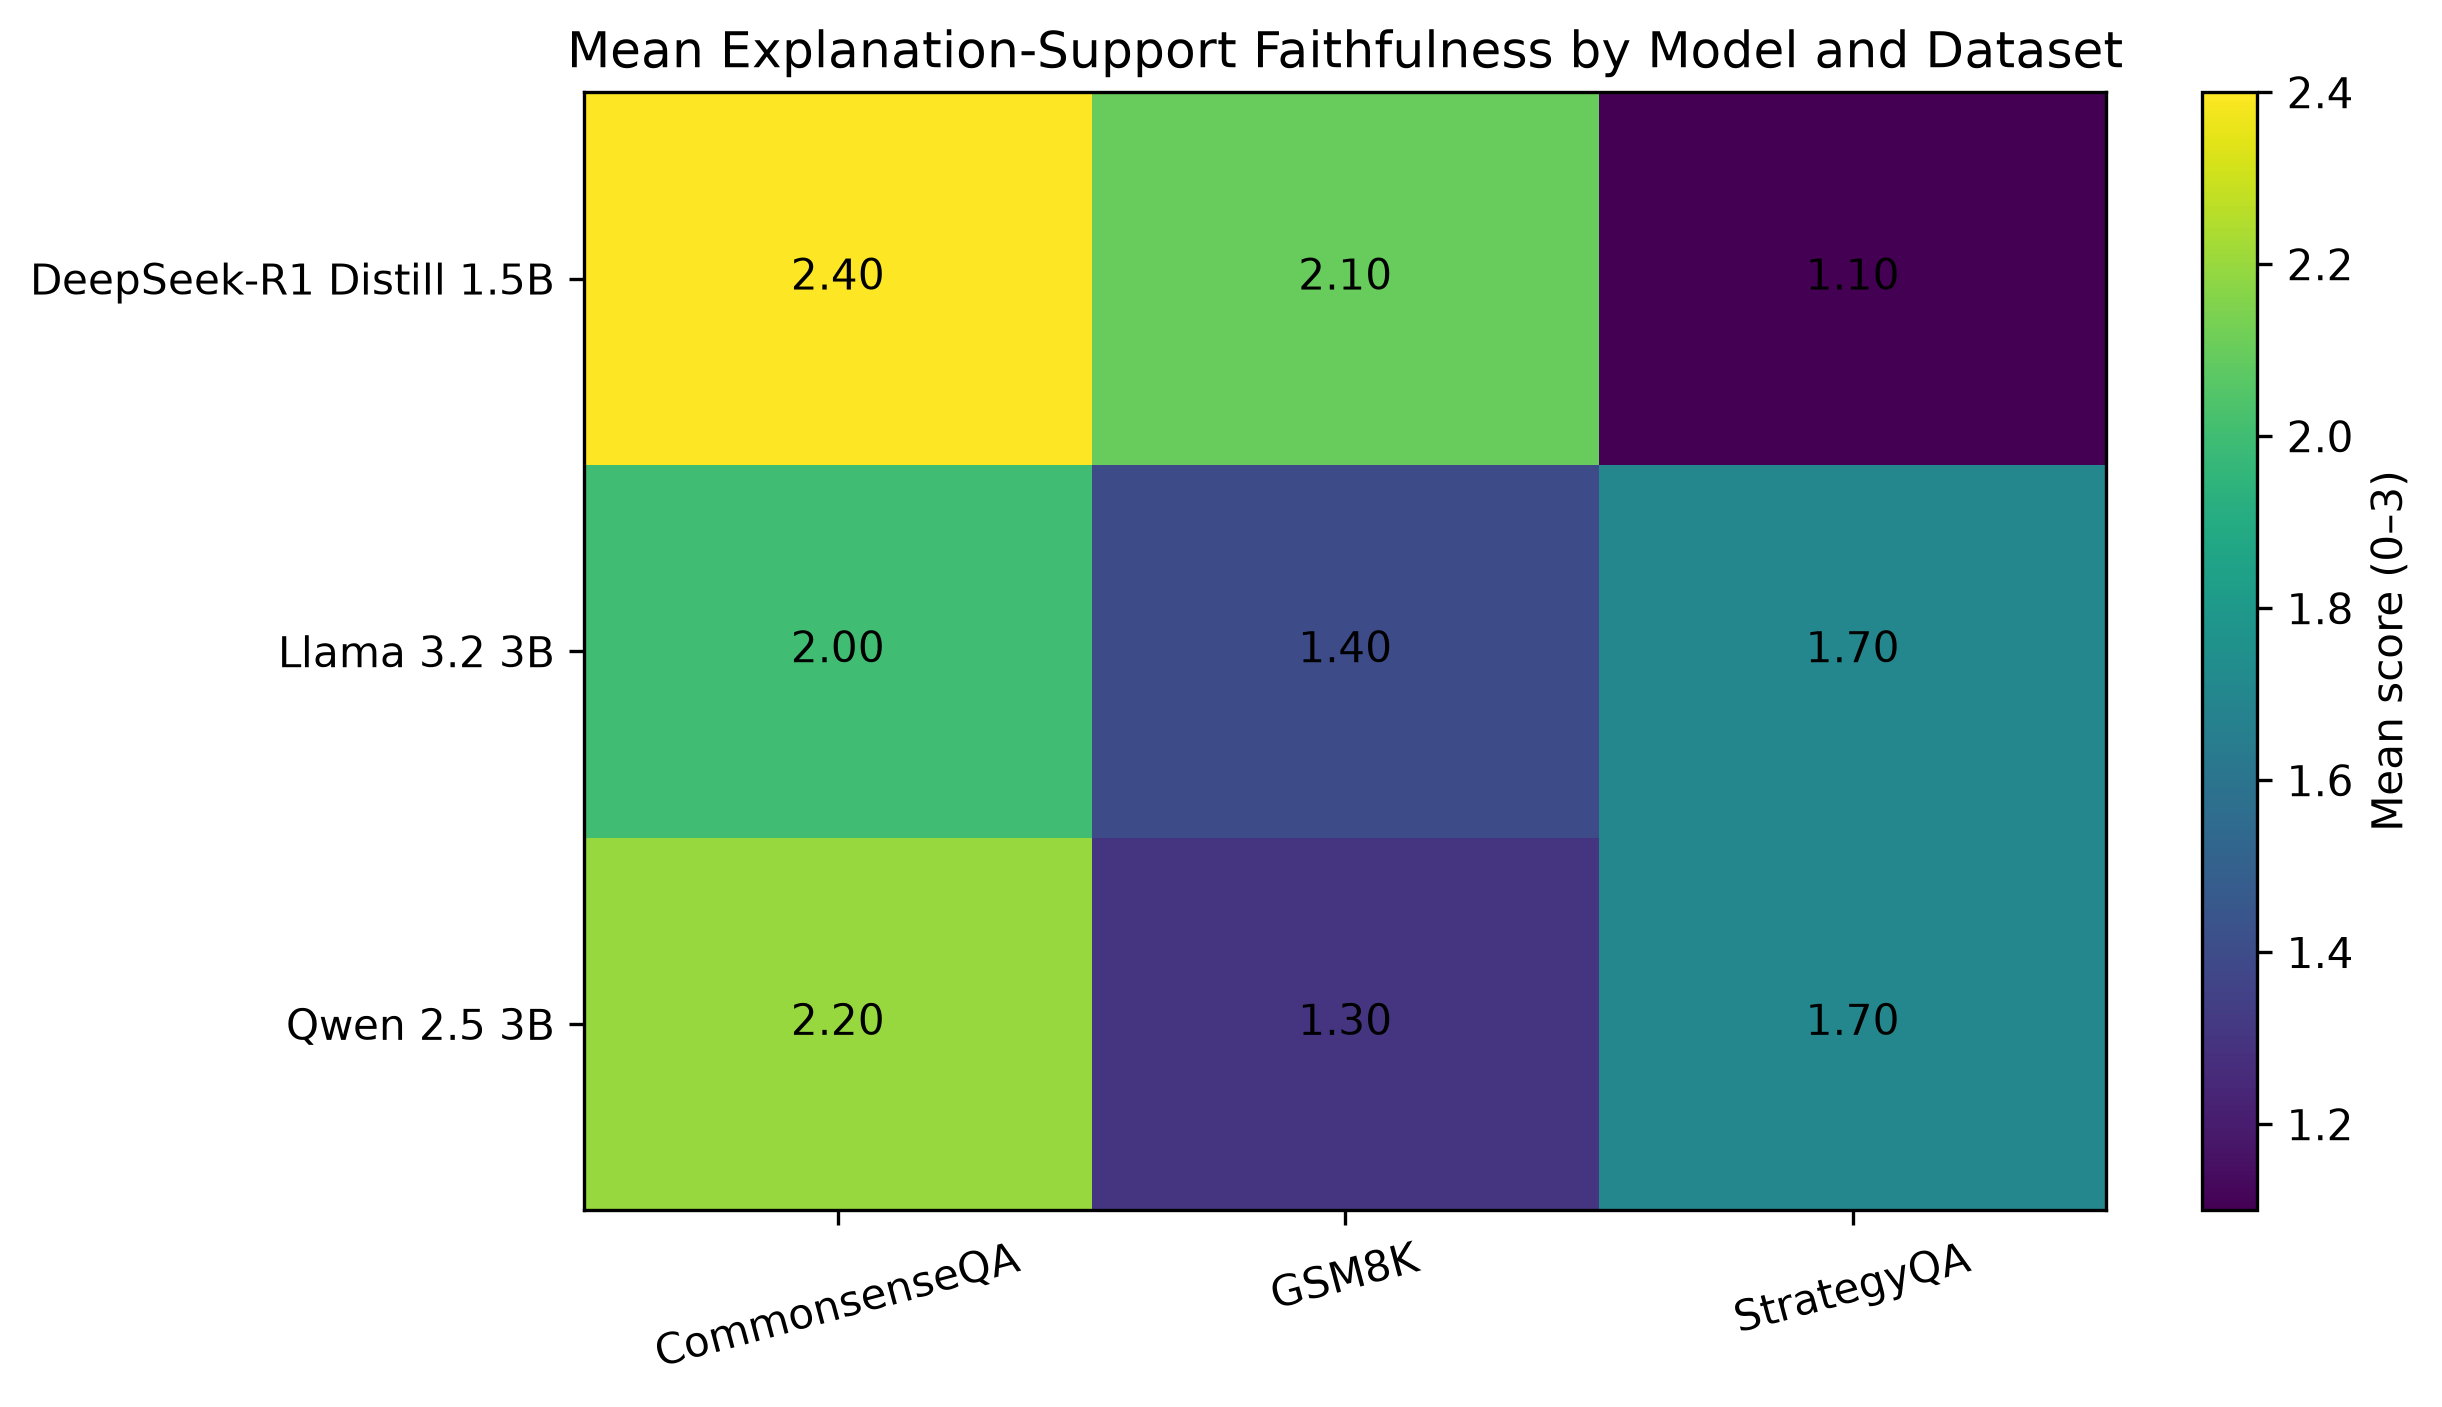
\includegraphics[width=\linewidth]{faithfulness_heatmap.png}
    \caption{Mean explanation-support faithfulness by model and dataset.
    The values show substantial task-dependent variation.}
    \label{fig:appendix_heatmap}
\end{figure}

\begin{figure}[t]
    \centering
    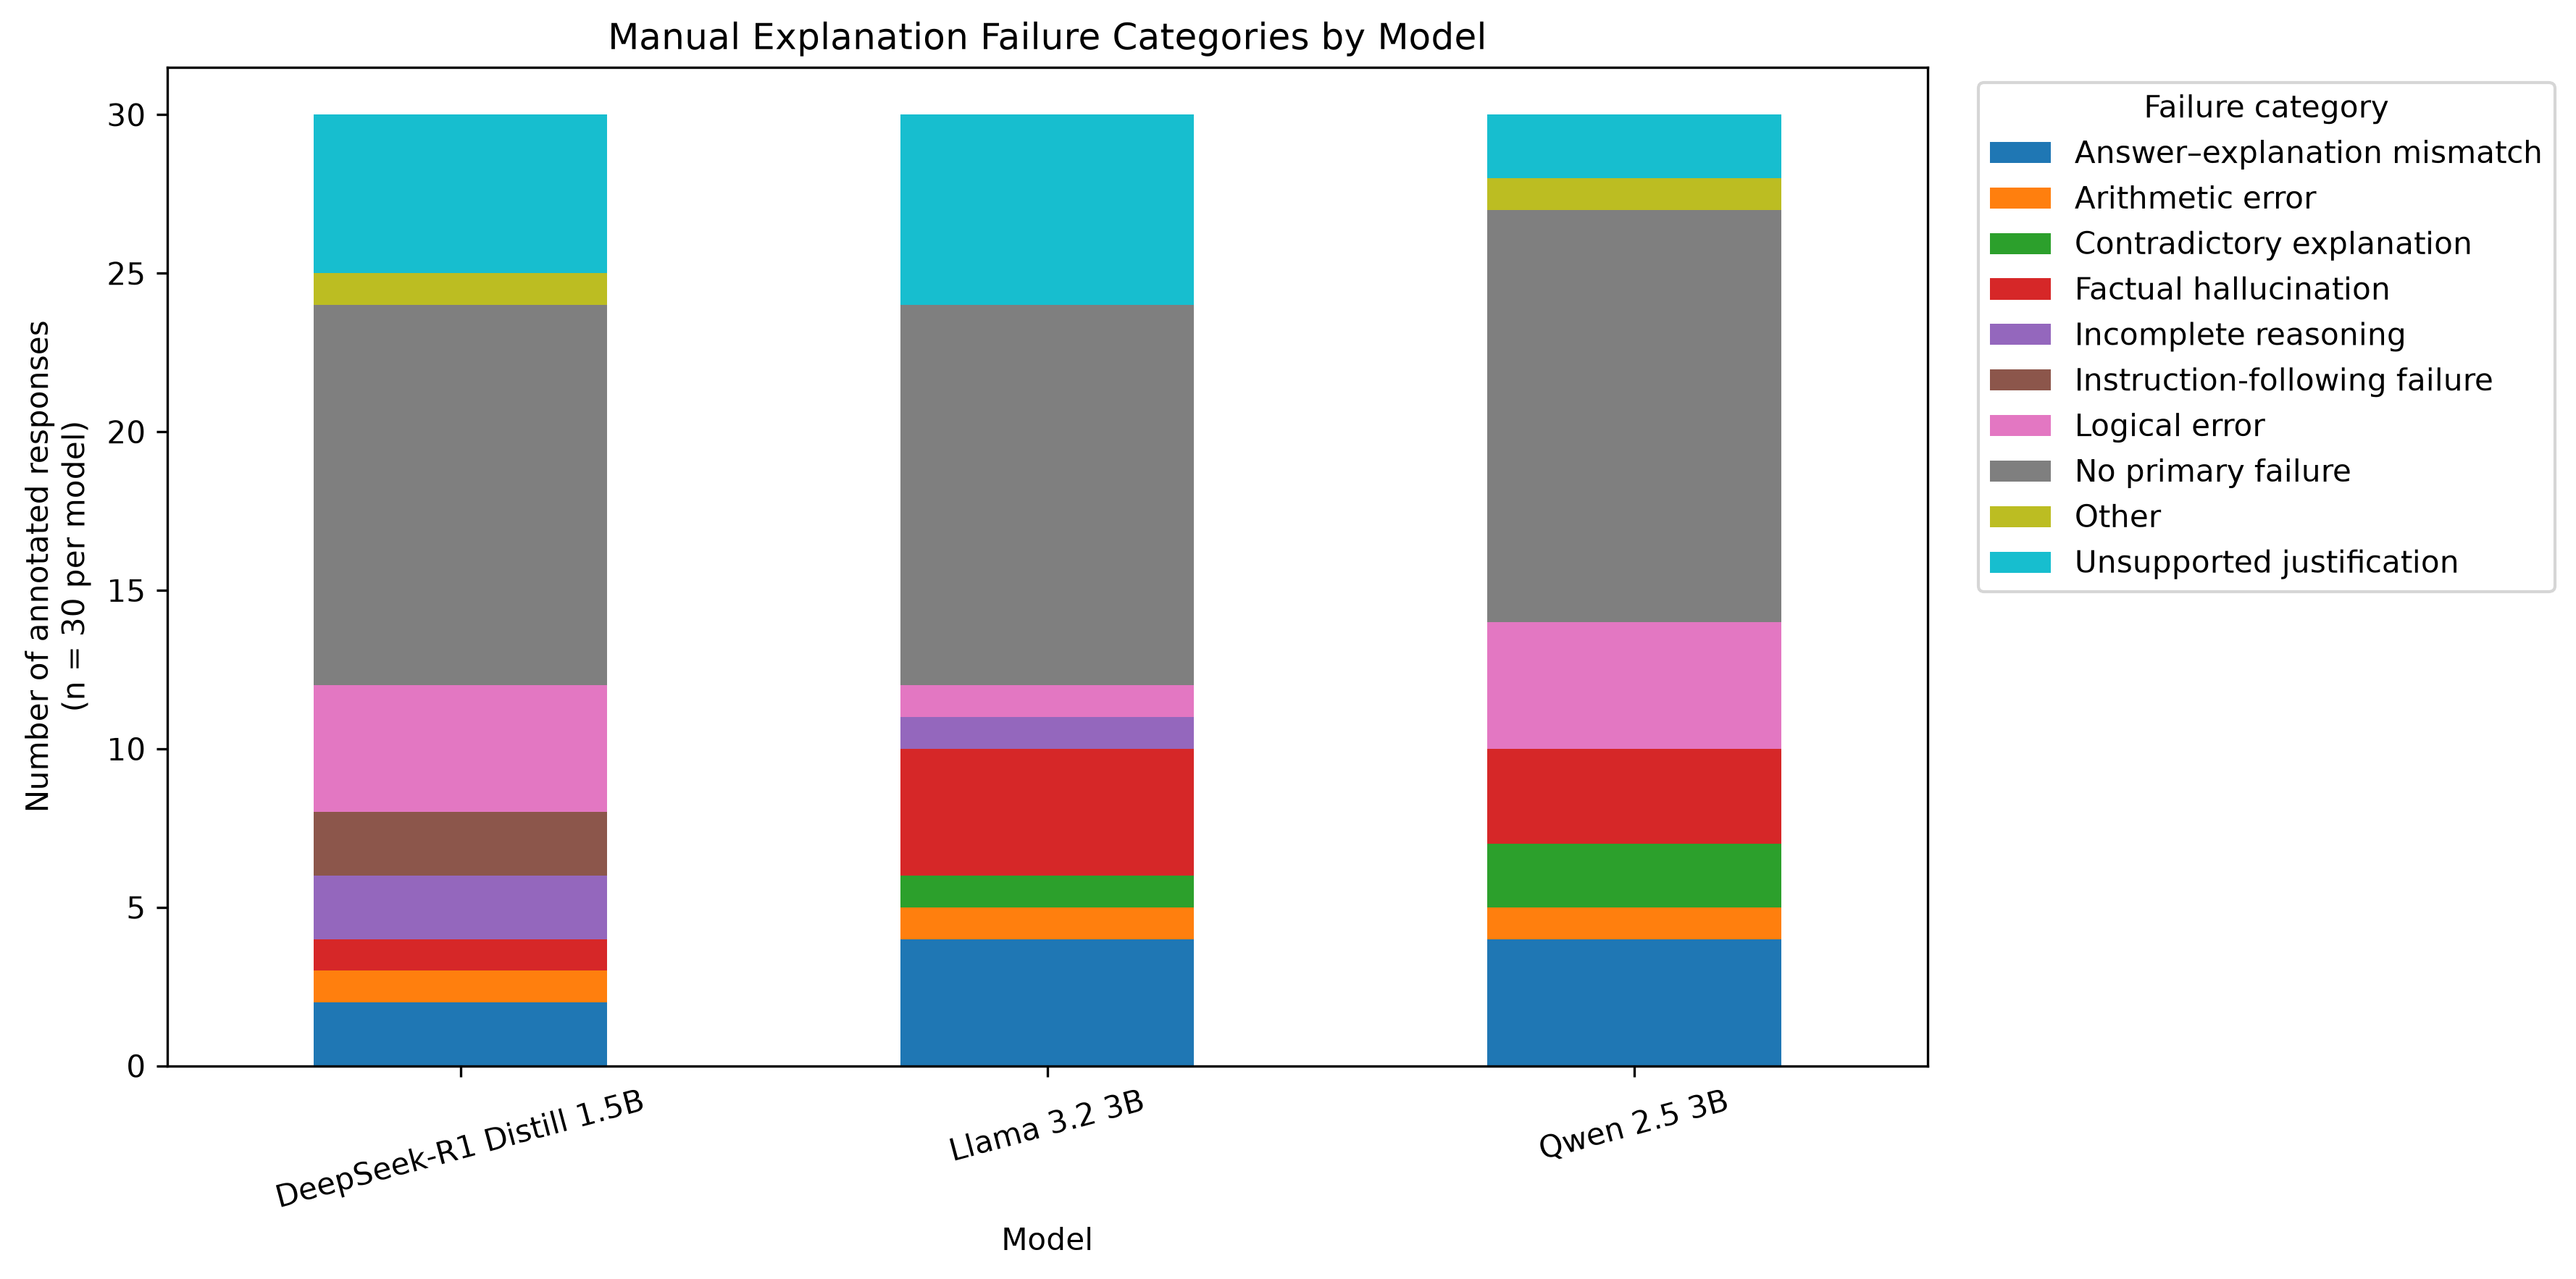
\includegraphics[width=\linewidth]{failure_categories_by_model.png}
    \caption{Primary explanation failure categories in the balanced
    manual-analysis sample ($n=30$ per model).}
    \label{fig:appendix_failures}
\end{figure}

The heatmap shows that DeepSeek obtained the highest mean faithfulness on
CommonsenseQA (2.40) and GSM8K (2.10), but the lowest score on StrategyQA
(1.10). Llama obtained 2.00 on CommonsenseQA, 1.40 on GSM8K, and 1.70 on
StrategyQA. Qwen obtained 2.20, 1.30, and 1.70, respectively.

The failure-category figure shows that unsupported justification was common for
DeepSeek and Llama. Llama and Qwen also exhibited factual hallucinations and
answer--explanation mismatches, while Qwen additionally produced contradictory
explanations.

\section{Qualitative Examples}
\label{app:qualitative}

Table~\ref{tab:qualitative_examples} presents representative examples from the
reviewed manual-analysis sample. Excerpts are shortened for readability.

\begin{table*}[t]
\centering
\scriptsize
\caption{Representative qualitative examples from the reviewed sample.}
\label{tab:qualitative_examples}
\begin{tabular}{p{2.0cm}p{1.4cm}p{2.0cm}p{1.3cm}p{1.3cm}p{5.7cm}p{2.4cm}}
\toprule
\textbf{Model} &
\textbf{Dataset} &
\textbf{Case} &
\textbf{Gold} &
\textbf{Prediction} &
\textbf{Explanation excerpt} &
\textbf{Primary failure} \\
\midrule

DeepSeek-R1 Distill 1.5B &
CommonsenseQA &
Strong correct explanation &
E. tiredness &
E &
Tiredness is likely because running after a ball requires exerting energy,
leading to fatigue. &
None \\

Llama 3.2 3B &
GSM8K &
Answer--explanation mismatch &
720 &
960 &
Greta first puts 50\% of her \$2400 paycheck into retirement, which is
\$1200. She then uses 20\% of the paycheck for her car payment, which is
\$480. &
Answer--explanation mismatch \\

Qwen 2.5 3B &
CommonsenseQA &
Unsupported justification &
D. outside &
C. windowsill &
Ivy plants often require sunlight, which they can receive from warm
south- or west-facing windowsills. Windowsills also provide a stable
surface. &
Unsupported justification \\

Llama 3.2 3B &
StrategyQA &
Factual hallucination &
No &
B &
A modern CPU circuit chip is typically quite large and bulky, often
measuring several inches in size, whereas a house key is small and thin. &
Factual hallucination \\

DeepSeek-R1 Distill 1.5B &
GSM8K &
Logical or arithmetic error &
525 &
580 &
Andy needs to burn 105,000 calories over 181 days, which averages to
approximately 580 calories per day. &
Logical error \\
\bottomrule
\end{tabular}
\end{table*}

These examples illustrate that explanation fluency does not guarantee that the
reasoning is correct, complete, or aligned with the final answer.

\section{Reproducibility Details}
\label{app:reproducibility}

The final processed benchmark contained 300 questions and used random seed 42.
It was stored in both CSV and JSONL formats.

The SHA-256 checksum of the final processed benchmark CSV was:

\begin{quote}
\small
\texttt{35b721529e523d4a945407053ded18d93489e5476a23ec90fad1923fb36906e5}
\end{quote}

The complete experiment generated:

\[
3\ \text{models}
\times
3\ \text{datasets}
\times
100\ \text{samples}
=
900\ \text{responses}.
\]

Generated records preserved:

\begin{itemize}
    \item model identifier;
    \item dataset and sample identifier;
    \item complete prompt;
    \item raw generation;
    \item parsed final answer;
    \item extracted explanation;
    \item ground-truth answer;
    \item correctness label;
    \item generation time;
    \item strict parse status;
    \item processing error field.
\end{itemize}

Generated outputs were written incrementally to JSONL files so interrupted
runs could resume without regenerating completed samples. Model outputs were
evaluated separately by dataset and then merged into model-level and
cross-model result tables.

\section{Reproduction Commands}
\label{app:commands}

The main stages of the project were executed using commands of the following
form:

\begin{verbatim}
python -m src.prepare_data
python -m src.inspect_data
python -m src.run_inference
python -m src.evaluate_answers
python -m src.combine_results
python -m src.select_balanced_annotations
python -m src.analyze_manual_annotations
python -m src.statistical_analysis
python -m src.select_qualitative_examples
python -m src.create_paper_figures
\end{verbatim}

The exact model, dataset, input, output, token-budget, and overwrite arguments
are preserved in the project scripts and configuration files.



\end{document}